\documentclass[11pt]{report}

% Dependencies
\usepackage{graphicx}
\usepackage{amsmath}
\usepackage{multicol}
\usepackage{amssymb}
\usepackage{tabularx}
\usepackage{xcolor}
\usepackage{fancyhdr}
\usepackage{fontspec}
\usepackage{titlesec, blindtext}
\usepackage[spanish,es-tabla]{babel}
\usepackage{tocloft}
\usepackage[
    hyperindex=true,
    bookmarks=true,
    bookmarksnumbered=true,
    hidelinks,
]{hyperref}
\usepackage[all]{hypcap}

%%%%%%%%%%%%%%%%%%%%%%%%%%%%%%%%%%%%%%%%%%%%%%%%%%%%%%%%%%%%%%%%%%%%%%%%%%%%%%%
% Document style                                                              %
%%%%%%%%%%%%%%%%%%%%%%%%%%%%%%%%%%%%%%%%%%%%%%%%%%%%%%%%%%%%%%%%%%%%%%%%%%%%%%%

\usepackage[
    lmargin=3cm,
    rmargin=3cm,
    tmargin=2.5cm,
    bmargin=2.5cm,
]{geometry}
\setmainfont{Arial}
\definecolor{greyed}{RGB}{242,242,242}

\fancypagestyle{plain}{
    \setlength{\headheight}{18.18pt}
    \fancyhf{}
    \fancyhead[L]{
        \color{gray}
        \scriptsize
        Desarrollo de una herramienta de análisis de tráfico de red y su uso en algoritmos de ML para la detección de ataques.
        \\
        Raul Rabadan Arroyo
    }
    %\renewcommand{\headrulewidth}{0pt}
    \fancyfoot[R]{\thepage}
}
\pagestyle{plain}

\fancypagestyle{nonumber}{
    \fancyhf{}
    \renewcommand{\headrulewidth}{0pt}
}

\titleformat{\chapter}[hang]{\huge\bfseries}{\theHchapter.~}{0pt}{\huge\bfseries}
\titlespacing*{\chapter}{0pt}{0pt}{12pt}

\renewcommand{\baselinestretch}{1.5} 

\bibliographystyle{plain}
\addto\captionsspanish{\renewcommand{\bibname}{BIBLIOGRAFÍA}}

%%%%%%%%%%%%%%%%%%%%%%%%%%%%%%%%%%%%%%%%%%%%%%%%%%%%%%%%%%%%%%%%%%%%%%%%%%%%%%%
% Table of contents style                                                     %
%%%%%%%%%%%%%%%%%%%%%%%%%%%%%%%%%%%%%%%%%%%%%%%%%%%%%%%%%%%%%%%%%%%%%%%%%%%%%%%

\tocloftpagestyle{empty}

% Table of contents title
\setlength{\cftbeforetoctitleskip}{0ex}%
\setlength{\cftaftertoctitleskip}{0ex}%
\renewcommand{\cfttoctitlefont}{\hfill\textbf}%
\renewcommand{\cftaftertoctitle}{\hfill}%
\addto\captionsspanish{\renewcommand{\contentsname}{ÍNDICE}}

% Table of contents chapter
\setlength{\cftbeforechapskip}{1em}%
\setlength{\cftchapindent}{0em}%
\renewcommand{\cftchapaftersnum}{. \space}%
\renewcommand{\cftchapleader}{\hfill}%

% Table of contents section
\setlength{\cftbeforesecskip}{0.5em}%
\setlength{\cftsecindent}{0em}%
\renewcommand{\cftsecfont}{\bfseries\footnotesize}%
\renewcommand{\cftsecpagefont}{\bfseries\footnotesize}%
\renewcommand{\cftsecaftersnum}{. \space}%
\renewcommand{\cftsecleader}{\hfill}%

% Table of contents subsection
\setlength{\cftbeforesubsecskip}{0.5em}%
\setlength{\cftsubsecindent}{0em}%
\renewcommand{\cftsubsecfont}{\bfseries\footnotesize}%
\renewcommand{\cftsubsecpagefont}{\bfseries\footnotesize}%
\renewcommand{\cftsubsecaftersnum}{. \space}%
\renewcommand{\cftsubsecleader}{\hfill}%

% Table of contents subsubsection
\setlength{\cftbeforesubsubsecskip}{0.5em}%
\setlength{\cftsubsubsecindent}{0em}%
\renewcommand{\cftsubsubsecfont}{\bfseries\footnotesize}%
\renewcommand{\cftsubsubsecpagefont}{\bfseries\footnotesize}%
\renewcommand{\cftsubsubsecaftersnum}{. \space}%
\renewcommand{\cftsubsubsecleader}{\hfill}%

% List of figures title
\setlength{\cftbeforeloftitleskip}{0ex}%
\setlength{\cftafterloftitleskip}{0ex}%
\renewcommand{\cftloftitlefont}{\hfill\textbf}%
\renewcommand{\cftafterloftitle}{\hfill}%
\addto\captionsspanish{\renewcommand{\listfigurename}{ÍNDICE DE FIGURAS}}

% List of figures point
\renewcommand{\cftfigleader}{\hfill}%
\setlength{\cftfignumwidth}{5em}
\renewcommand{\cftfigpresnum}{Figura~}
\renewcommand{\cftfigaftersnum}{.}

% List of tables title
\setlength{\cftbeforelottitleskip}{0ex}%
\setlength{\cftafterlottitleskip}{0ex}%
\renewcommand{\cftlottitlefont}{\hfill\textbf}%
\renewcommand{\cftafterlottitle}{\hfill}%
\addto\captionsspanish{\renewcommand{\listtablename}{ÍNDICE DE TABLAS}}

% List of tables point
\renewcommand{\cfttableader}{\hfill}%
\setlength{\cfttabnumwidth}{5em}
\renewcommand{\cfttabpresnum}{Tabla~}
\renewcommand{\cfttabaftersnum}{.}

%%%%%%%%%%%%%%%%%%%%%%%%%%%%%%%%%%%%%%%%%%%%%%%%%%%%%%%%%%%%%%%%%%%%%%%%%%%%%%%
% Glossary                                                                    %
%%%%%%%%%%%%%%%%%%%%%%%%%%%%%%%%%%%%%%%%%%%%%%%%%%%%%%%%%%%%%%%%%%%%%%%%%%%%%%%

% Import
\usepackage[acronym,automake,section=subsubsection]{glossaries}

% Generation
\makeglossaries

% Contents
\newglossaryentry{matrix}% the label
{name={matrix},% the term
 description={a rectangular table of elements},% brief description
 plural={matrices}% the plural
}

\newglossaryentry{userdatagramprotocol}% the label
{name={User Datagram Protocol},% the term
 description={Protocolo de red de la capa de transportes orientado a mensajes.},% brief description
}

\newacronym{ml}{ML}{Machine learning}
\newacronym{udp}{UDP}{User Datagram Protocol}

% Style

\addto\captionsspanish{\renewcommand{\glossaryname}{TÉRMINOS}}
\addto\captionsspanish{\renewcommand{\acronymname}{ACRÓNIMOS}}

%%%%%%%%%%%%%%%%%%%%%%%%%%%%%%%%%%%%%%%%%%%%%%%%%%%%%%%%%%%%%%%%%%%%%%%%%%%%%%%
% Document                                                                    %
%%%%%%%%%%%%%%%%%%%%%%%%%%%%%%%%%%%%%%%%%%%%%%%%%%%%%%%%%%%%%%%%%%%%%%%%%%%%%%%

\begin{document}

% Front pages
\selectlanguage{spanish}
\begin{titlepage}
    
\includegraphics{media/epsevg_logo.jpeg}
    \begin{center}

        \vspace{1.5cm}
        {\Huge\textbf{TRABAJO FINAL DE GRADO}}

        \vfill
        ~\\ % Empty line so its aligned to the appendices

        \vfill

        \setlength\fboxsep{0.5cm}\fbox{
            \parbox{13.5cm}{
                \par{
                    \textbf{TÍTULO:} \MakeUppercase[]{Desarrollo de una herramienta de análisis de tráfico de red y su uso en algoritmos de ML para la detección de ataques.}
                    \\[\baselineskip]
                    \textbf{AUTOR:} RABADAN ARROYO, RAUL
                    \\[\baselineskip]
                    \textbf{FECHA DE PRESENTACIÓN:} JULIO, 2024
                }
            }
        }

        \vfill

    \end{center}
\end{titlepage}

\begin{titlepage}
    \begin{center}
        \setlength\fboxsep{0.5cm}\fbox{
            \parbox{13.5cm}{
                \par{
                    \textbf{APELLIDOS:} RABADAN ARROYO \quad \textbf{NOMBRE:} RAUL \\[\baselineskip]
                    \textbf{TITULACIÓN:} GRADO EN INGENIERÍA INFORMÁTICA \\[\baselineskip]
                    \textbf{PLAN:} 2018 \\[\baselineskip]
                    \textbf{DIRECTORA:} SIMO MEZQUITA, ESTER \\[\baselineskip]
                    \textbf{DEPARTAMENTO:} DEPARTAMENTO DE MATEMÁTICAS
                }
            }
        }
    \end{center}
    
    \vfill

    \begin{center}
        \setlength\fboxsep{0cm}\colorbox{greyed}{\setlength\fboxsep{0.5cm}\fbox{
            \parbox[t]{7.5cm}{
                \centering{
                    \textbf{CALIFICACIÓN DEL TFG}
                }
                \vspace {
                    2cm
                }
            }
        }}
    \end{center}

    \vfill

    \begin{center}
        \setlength\fboxsep{0cm}\colorbox{greyed}{\setlength\fboxsep{0.5cm}\fbox{
            \parbox{13.5cm}{
                \begin{center}
                    \underline{
                        \textbf{
                            TRIBUNAL
                        }
                    }
                \end{center}
                
                \hspace{1cm}
                \textbf{PRESIDENTE}
                \hfill
                \textbf{SECRETARIO}
                \hfill
                ~~ % Make it the same with as the others
                \textbf{VOCAL}
                ~~~ % Make it the same with as the others
                \hspace{1.3cm}

                \vspace {
                    3cm
                }
                \hspace{0.9cm}
                \textbf{FECHA DE LECTURA:}
                \vspace {
                    0.5cm
                }
            }
        }}
    \end{center}

    \vfill

    \begin{center}
        \textbf{
            Este proyecto tiene en cuenta aspectos medioambientales: \square ~ Sí ~ \blacksquare ~ No
        }
    \end{center}
    
\end{titlepage}

% Abatracts
\selectlanguage{spanish}
\newpage
\pagestyle{nonumber}

\begin{center}
    \textbf{
        RESUMEN
    }
    \\[\baselineskip]
\end{center}

\begin{center}
    \setlength\fboxsep{0.05\textwidth}\fbox{
        \parbox[t][\textwidth]{0.8\textwidth}{
            \quad \quad En este trabajo se hace el desarrollo de una herramienta de análisis de red y se demuestra su funcionamiento a partir de analizar trazas de tráfico de red y su uso en algoritmos de Machine Learning.
            
            \quad \quad Para el desarrollo de la herramienta se ha hecho uso de Rust y en las tareas de Machine Learning y análisis de datos se ha trabajado con Python. El desarrollo se ha realizado bajo un entorno de desarrollo en un contenedor Docker. Todo el código de la herramienta, los scripts y la configuración del entorno se ofrecen para permitir resultados lo más reproducibles posibles.
            
            \quad \quad La herramienta es capaz de generar 72 características continuas con información de flujos TCP y UDP, además de 2 discretas indicando el protocolo de transporte y una identificación de cada flujo compuesta por 7 valores. Adicionalmente, la herramienta permite realizar un etiquetado automático a partir de un fichero CSV en el cual se indica por cada fila el par de direcciones IP, el protocolo de transporte utilizado y el tiempo de inicio y 
            final.
            
            \quad \quad A partir de los conjuntos de datos utilizados, la herramienta desarrollada y un modelo basado en bosques aleatorios, se ha obtenido un valor de precisión del 99.95\% y una puntuación F1 media del 98.66\%
            
            \quad \quad La herramienta desarrollada puede ser utilizada como componente en sistemas  de detección de intrusiones y tiene el potencial para ser extendida con más funcionalidades en el futuro.
        }
    }
\end{center}

\vspace{0.3cm}
\textbf{Palabras clave:}
\begin{center}
    \renewcommand{\arraystretch}{1.5}\begin{tabular}{|m{0.2\textwidth}|m{0.2\textwidth}|m{0.2\textwidth}|m{0.2\textwidth}|}
        \hline
            \centering\arraybackslash{Análisis de red} & \centering\arraybackslash{Machine Learning} & \centering\arraybackslash{Ciberseguridad} & \centering\arraybackslash{Desarrollo} \\
        \hline
        \centering\arraybackslash{Python} & \centering\arraybackslash{Rust} & \centering\arraybackslash{Docker} \\
        \cline{1-3}
    \end{tabular}
\end{center}

\selectlanguage{catalan}
\newpage
\pagestyle{nonumber}

\begin{center}
    \textbf{
        RESUM
    }
    \\[\baselineskip]
\end{center}

\begin{center}
    \setlength\fboxsep{0.05\textwidth}\fbox{
        \parbox[t][\textwidth]{0.8\textwidth}{
            \par{
                Amb una extensió màxima de 50 línies, i amb una llista de màxim 10 paraules clau, el resum és un text informatiu que permet decidir sobre la utilitat de llegir el document complet; ha de definir l’objectiu, els mètodes, els resultats i les conclusions presentats en el cos del document, en aquest ordre o destacant inicialment els resultats i les conclusions; ha de ser un text complet perquè sigui intel·ligible sense necessitat de referir-se a la memòria; ha de contenir la informació bàsica i el caràcter del document original. Com en tots els documents cal vetllar per la correcció d’estil, cal també emprar una nomenclatura normalitzada, i definir els termes no familiars les abreviacions i els símbols, quan apareguin per primera vegada en el resum. És la pàgina número 1 del document.
            }
        }
    }
\end{center}

\vspace{0.3cm}
\textbf{Paraules clau (màxim 10):}
\begin{center}
    \renewcommand{\arraystretch}{1.5}\begin{tabular}{|m{0.2\textwidth}|m{0.2\textwidth}|m{0.2\textwidth}|m{0.2\textwidth}|}
        \hline
            \centering\arraybackslash{?} & \centering\arraybackslash{?} & \centering\arraybackslash{?} & \centering\arraybackslash{?} \\
        \hline
        \centering\arraybackslash{?} & \centering\arraybackslash{?} & \centering\arraybackslash{?} & \centering\arraybackslash{?} \\
        \hline
        \centering\arraybackslash{?} & \centering\arraybackslash{?} \\
        \cline{1-2}
    \end{tabular}
\end{center}

\selectlanguage{english}
\newpage
\pagestyle{nonumber}

\begin{center}
    \textbf{
        ABSTRACT
    }
    \\[\baselineskip]
\end{center}

\begin{center}
    \setlength\fboxsep{0.05\textwidth}\fbox{
        \parbox[t][\textwidth]{0.8\textwidth}{
            \quad \quad This project contains the development of a network analysis tool, the showcase of its usage on network traces, and the employment of the results on Machine Learning algorithms.

            \quad \quad Rust has been used for the development of the tool and Python for the data analysis process and Machine Learning. The development has been made in a containerized development environment. All the code from the tool, the scripts and the configuration of the environment are available to allow for reproducible results.
            
            \quad \quad The tool is capable of generating 72 continuous features with information about the TCP and UDP flows. In addition to the previous, it adds 2 discrete columns to indicate the used protocol and 7 values to be able to identify each detected flow. Additionally, the tool allows the user to provide a \acrshort{csv} file in order to perform automatic tagging. This file should contain, for each record, the pair of IP addresses, the used transport protocol, and the starting and ending timestamps.
            
            \quad \quad With the source datasets, the developed tool and a model based on random forests, a precision value of 99.95\% and an average F1 macro score of 98.66\% were obtained.
            
            \quad \quad The tool can be used as a component in an intrusion detection system and has the possibility to be extended with more functionalities in the future.
        }
    }
\end{center}

\vspace{0.3cm}
\textbf{Keywords:}
\begin{center}
    \renewcommand{\arraystretch}{1.5}\begin{tabular}{|m{0.2\textwidth}|m{0.2\textwidth}|m{0.2\textwidth}|m{0.2\textwidth}|}
        \hline
            \centering\arraybackslash{Network analysis} & \centering\arraybackslash{Machine Learning} & \centering\arraybackslash{Cybersecurity} & \centering\arraybackslash{Development} \\
        \hline
        \centering\arraybackslash{Python} & \centering\arraybackslash{Rust} & \centering\arraybackslash{Docker} \\
        \cline{1-3}
    \end{tabular}
\end{center}


% Indices
\selectlanguage{spanish}
\selectlanguage{spanish}
\tableofcontents
\newpage
\listoffigures
\newpage
\listoftables
\newpage
\setglossarystyle{index}
%\hfill\textbf{GLOSARIO}\hfill
\printglossaries


% Contents
\newpage
\pagestyle{plain}

\phantomsection\addcontentsline{toc}{chapter}{INTRODUCCIÓN}
\chapter*{INTRODUCCIÓN}

La ciberseguridad es una de las fronteras del conocimiento que ha tomado más relevancia estos últimos años. Para salvaguardar la disponibilidad, integridad y confidencialidad de la información tanto almacenada como en tránsito, se aplican numerosas y diversas técnicas en conjunto. Desde medidas criptográficas para proteger la información hasta el análisis del tráfico de red para detectar comportamientos maliciosos y poder bloquearlos. El presente trabajo se focalizará en el último punto.

\phantomsection\addcontentsline{toc}{section}{MOTIVACIÓN}
\section*{MOTIVACIÓN}

La motivación de este trabajo radica en mi interés por la aplicabilidad de los sistemas de \gls{ml} en entornos limitados o con requerimientos de actuación en tiempo real, especialmente en el ámbito de ciberseguridad en las redes. En muchos casos, los tráficos de red maliciosos son identificados cuando estos ya han ocurrido o están generando problemas activamente para el resto de usuarios de la red La hazaña intelectual que supondría la detección de ataques en su inicio o incluso antes de que ocurriesen es una meta en la que me gustaría colaborar. Llegar a este ideal es seguramente improbable. Sin embargo, tenerlo como horizonte para dirigir el camino y acercarse lo máximo posible a este, ofrece la capacidad de mejorar la mitigación contra posibles adversarios.

Existen diversas herramientas similares a la ideada para el trabajo, pero debido a su dificultad de uso, su naturaleza propietaria o su desalineación al uso específico que se le quiere dar, he querido desarrollar una alternativa.

\phantomsection\addcontentsline{toc}{section}{OBJETIVOS}
\section*{OBJETIVOS}

El objetivo principal del trabajo consiste en diseñar, programar y demostrar la utilidad de una herramienta de análisis de red basada en la extracción de características de esta para detectar comportamientos maliciosos. La herramienta requerirá de ser robusta y eficiente, además de fácil de utilizar, extender y modificar. La robusteza y eficiencia son necesarias, ya que por su naturaleza tendrá que tratar datos en tiempo real en entornos limitados. La facilidad de uso, extensión y modificación es importante, ya que en el desarrollo de aplicaciones, y especialmente en el ámbito de la ciberseguridad, el entorno y los requerimientos están en constante variación.

La utilidad de la herramienta se evaluará según su capacidad de adaptación a diferentes entornos de ejecución y diferentes tipos de tráfico de red. Esto es necesario, ya que, dependiendo de su rendimiento, podrá ser integrada en sistemas más generales y complejos.

\phantomsection\addcontentsline{toc}{section}{METODOLOGÍA}
\section*{METODOLOGÍA}

(extreme programming, definir tests y metas etc)
\newpage
\pagestyle{plain}

\chapter{MARCO TEÓRICO}

\section{Anàlisis herramientas de extracción de características}

\subsection{CICFlowmeter}

CICFlowMeter es una herramienta para generar y analizar flujos de red \cite{cicflowpost}. Permite obtener información sobre flujos bidireccionales sobre IP, utilizen estos TCP o UDP. Por cada flujo, genera seis columnas identificativas y añade cierta información del flujo. En el Readme del codigo fuente ofrecido, podemos encontrar las características generades.

\begin{itemize}
    \item \textbf{Flow ID}: Combinación de las otras columnas separadas por giones
    \item \textbf{Src IP}: La dirección IP del remitente des de la cual se ha iniciado el flujo
    \item \textbf{Src Port}: La dirección IP del destinatario hacia la cual se ha dirigido el flujo
    \item \textbf{Dst IP}: El puerto origen o de retorno del remitente
    \item \textbf{Dst Port}: El puerto destino del destinatario
    \item \textbf{Protocol}: Identificador del protocolo sobre IP segun definido por IANA \cite{ipprotocolnumbers}
    \item \textbf{Timestamp}: Momento del incio del flujo, expresado en dd/MM/yyyy hh:mm:ss de la zona horaria local. En la descripción se indica que 
    \item \textbf{Flow Duration}: Duracion del flujo, expresado en microsegundos
    \item \textbf{Total Fwd Packet}: Número total de paquetes hacia el destinatario
    \item \textbf{Total Bwd packets}: Número total del paquetes hacia el receptor
    \item \textbf{Total Length of Fwd Packet}: Número completo de bytes transmitidos hacia el destinatario
    \item \textbf{Total Length of Bwd Packet}: Número completo de bytes recibidos des del destinatario
    \item \textbf{Fwd Packet Length Max}: Tamaño en bytes del paquete mas grande enviado hacia el destinatario
    \item \textbf{Fwd Packet Length Min}: Tamaño en bytes del paquete mas pequeño enviado hacia el destinatario
    \item \textbf{Fwd Packet Length Mean}: Media aritmética del tamaño en bytes de los paquetes enviados hacia el destinatario
    \item \textbf{Fwd Packet Length Std}: Desviación estándard del tamaño en bytes de los paquetes enviados hacia el destinatario
    \item \textbf{Bwd Packet Length Max}: Tamaño en bytes del paquete mas grande enviado hacia el emisor
    \item \textbf{Bwd Packet Length Min}: Tamaño en bytes del paquete mas pequeño enviado hacia el emisor
    \item \textbf{Bwd Packet Length Mean}: Media aritmética del tamaño en bytes de los paquetes enviados hacia el emisor
    \item \textbf{Bwd Packet Length Std}: Desviación estándard del tamaño en bytes de los paquetes enviados hacia el emisor
    \item \textbf{Flow Bytes s}: Bytes por segundo del flujo
    \item \textbf{Flow Packets s}: Paquetes por segundo del flujo
    \item \textbf{Flow IAT Mean}: Media aritmética del tiempo de llegada entre paquetes
    \item \textbf{Flow IAT Std}: Desviación estándard del tiempo de llegada entre paquetes
    \item \textbf{Flow IAT Max}: Tiempo máximo de llegada entre paquetes
    \item \textbf{Flow IAT Min}: Tiempo mínimo de llegada entre paquetes
    \item \textbf{Fwd IAT Total}: Tiempo total entre la llegada de dos paquetes hacia el receptor
    \item \textbf{Fwd IAT Mean}: Media aritmética del tiempo de llegada entre paquetes hacia el receptor
    \item \textbf{Fwd IAT Std}: Desviación estándard del tiempo de llegada entre paquetes hacia el receptor
    \item \textbf{Fwd IAT Max}: Tiempo máximo de llegada entre paquetes hacia el receptor
    \item \textbf{Fwd IAT Min}: Tiempo mínimo de llegada entre paquetes hacia el receptor
    \item \textbf{Bwd IAT Total}: Tiempo total entre la llegada de dos paquetes hacia el emisor
    \item \textbf{Bwd IAT Mean}: Media aritmética del tiempo de llegada entre paquetes hacia el emisor
    \item \textbf{Bwd IAT Std}: Desviación estándard del tiempo de llegada entre paquetes hacia el emisor
    \item \textbf{Bwd IAT Max}: Tiempo máximo de llegada entre paquetes hacia el emisor
    \item \textbf{Bwd IAT Min}: Tiempo mínimo de llegada entre paquetes hacia el emisor
    \item \textbf{Fwd PSH Flags}: Número de paquetes con el flag PSH activado en la cabecera TCP hacia el emisor
    \item \textbf{Bwd PSH Flags}: Número de paquetes con el flag PSH activado en la cabecera TCP hacia el receptor
    \item \textbf{Fwd URG Flags}: Número de paquetes con el flag URG activado en la cabecera TCP hacia el emisor
    \item \textbf{Bwd URG Flags}: Número de paquetes con el flag URG activado en la cabecera TCP hacia el receptor
    \item \textbf{Fwd Header Length}: Número de paquetes con el flag PSH activado en la cabecera TCP hacia el emisor
    \item \textbf{Bwd Header Length}: Número de paquetes con el flag PSH activado en la cabecera TCP hacia el receptor
    \item \textbf{Fwd Packets s}: Paquetes por segundo hacia el receptor
    \item \textbf{Bwd Packets s}: Paquetes por segundo hacia el emisor
    \item \textbf{Packet Length Min}: todo
    \item \textbf{Packet Length Max}: todo
    \item \textbf{Packet Length Mean}: todo
    \item \textbf{Packet Length Std}: todo
    \item \textbf{Packet Length Variance}: todo
    \item \textbf{FIN Flag Count}: todo
    \item \textbf{SYN Flag Count}: todo
    \item \textbf{RST Flag Count}: todo
    \item \textbf{PSH Flag Count}: todo
    \item \textbf{ACK Flag Count}: todo
    \item \textbf{URG Flag Count}: todo
    \item \textbf{CWR Flag Count}: todo
    \item \textbf{ECE Flag Count}: todo
    \item \textbf{Down Up Ratio}: todo
    \item \textbf{Average Packet Size}: todo
    \item \textbf{Fwd Segment Size.Avg}: todo
    \item \textbf{Bwd Segment Size Avg}: todo
    \item \textbf{Fwd Bytes Bulk Avg}: todo
    \item \textbf{Fwd Packet Bulk Avg}: todo
    \item \textbf{Fwd Bulk Rate Avg}: todo
    \item \textbf{Bwd Bytes Bulk Avg}: todo
    \item \textbf{Bwd Packet Bulk Avg}: todo
    \item \textbf{Bwd Bulk Rate Avg}: todo
    \item \textbf{Subflow Fwd Packets}: todo
    \item \textbf{Subflow Fwd Bytes}: todo
    \item \textbf{Subflow Bwd Packets}: todo
    \item \textbf{Subflow Bwd Bytes}: todo
    \item \textbf{FWD Init Win Bytes}: todo
    \item \textbf{Bwd Init Win Bytes}: todo
    \item \textbf{Fwd Act Data Pkts}: todo
    \item \textbf{Fwd Seg Size Min}: todo
    \item \textbf{Active Mean}: todo
    \item \textbf{Active Std}: todo
    \item \textbf{Active Max}: todo
    \item \textbf{Active Min}: todo
    \item \textbf{Idle Mean}: todo
    \item \textbf{Idle Std}: todo
    \item \textbf{Idle Max}: todo
    \item \textbf{Idle Min}: todo
\end{itemize}

\subsection{Wireshark}

a

\subsection{Zeek}

a

\subsection{ntopng}

a

\subsection{Argus}

a

\subsection{Softflowd}

a

\section{Datasets disponibles}

En esta sección analizaremos cuatro datasets disponibles utilizados para aplicaciones de ciberseguridad basadas en inteligencia artificial. Concretamente, observaremos CIC-DDos\-2019 \cite{8888419}, BoT-IoT \cite{DBLP:journals/corr/abs-1811-00701} \cite{10.1007/978-3-319-90775-8_3} \cite{KORONIOTIS202091} \cite{DBLP:journals/corr/abs-2005-00722} \cite{9252856} \cite{phdbotiot}, TON-IoT \cite{MOUSTAFA2021102994} \cite{9444348} \cite{9189760} \cite{9343133} \cite{9343084} \cite{moustafa2019systemic} \cite{ASHRAF2021103041} y UNSW-NB15 \cite{7348942} \cite{doi:10.1080/19393555.2015.1125974} \cite{7948715} \cite{Moustafa2017} \cite{10.1007/978-3-030-72802-1_9}.

\subsection{CICDDos2019}

\subsubsection{Descripción}

CICDDos2019 es un dataset creado por el Canadian Institute for Cybersecurity que contiene trazas de dos días en los que aparece tráfico benigno y serie de ataques DDoS típicos. \cite{cicddos2019web}. En este se contienen trazas de red en formato pcap y csvs con estadísticas de los flujos generados a partir de CICFlowMeter y posteriormente etiquetados. Para poder ofrecer un dataset público, realista y, además de mantener la privacidad de las comunicaciones originales, se generó tráfico sintético modelado a partir del comportamiento real de los usuarios. En las referencias se menciona el sistema utilizado para generar el comportamiento lo más natural posible de 25 usuarios haciendo uso de HTTP, HTTPS, FTP, SSH y protocolos de correo.

Los elementos de la red interna consisten en:

\begin{enumerate}
    \item Servidor web con Ubuntu 16.04 (192.168.50.1 en el primer día, 192.168.50.4 en el segundo día)
    \item Firewall con Fortinet (205.174.165.81)
    \item PC con Windows 7 (192.168.50.8 en el primer día, 192.168.50.9 en el segundo día)
    \item PC con Windows Vista (192.168.50.5 en el primer día, 192.168.50.6 en el segundo día)
    \item PC con Windows 8.1 (192.168.50.6 en el primer día, 192.168.50.7 en el segundo día)
    \item PC con Windows 10 (192.168.50.7 en el primer día, 192.168.50.8 en el segundo día)
\end{enumerate}

Adicionalmente, se han generado ataques DDoS basados en reflejos (usar un sistema de terceros para amplificar un ataque) y DDoS basado en exploits (tomar ventaja de vulnerabilidades en los protocolos). Según la información disponible \cite{cicddos2019web}, estos consisten en:

\begin{enumerate}
    \item \textbf{MSSQL}: Generado el primer día de 10:53 a 10:42 y el segundo de 11:36 a 11:45
    \item \textbf{SSDP}: Generado el segundo día de 12:27 a 12:37
    \item \textbf{DNS}: Generado el segundo día de 10:52 a 11:05
    \item \textbf{LDAP}: Generado el primer día de 10:21 a 10:30 y el segundo de 11:22 a 11:32
    \item \textbf{NetBIOS}: Generado el primer día de 10:00 a 10:09 y el segundo de 11:50 a 12:00
    \item \textbf{SNMP}: Generado el segundo día de 12:12 a 12:23
    \item \textbf{PortMap}: Generado el primer día de 9:43 a 9:51
    \item \textbf{WebDDoS}: Generado el segundo día de 13:18 a 13:29
    \item \textbf{NTP}: Generado el segundo día de 10:35 a 10:45
    \item \textbf{TFTP}: Generado el segundo día de 13:35 a 17:15
    \item \textbf{SYN Flood}: Generado el primer día de 11:28 a 17:35 y segundo día de 13:29 a 13:34
    \item \textbf{UDP Flood}: Generado el primer día de 10:53 a 11:03 y segundo día de 12:45 a 13:09
    \item \textbf{UDP-Lag}: Generado el primer día de 11:14 a 11:24 y segundo día de 13:11 a 13:15
\end{enumerate}

\subsubsection{Contenidos csvs}

El conjunto de datos procesados utilizando CICFlowMeter y etiquetado está compuesto por una lista de archivos por cada uno de los dos días en los que se generaron datos, el 3 de noviembre de 2018 y el 1 de diciembre de 2018. Las características ofrecidas son las mismas que las mencionadas en la herramienta CICFlowMeter. En todas las filas existen valores con excepción de algunas en la columna "Flow Bytes/s". Los scripts utilizados para la extracción y representación de los datos son \texttt{extract\_info\_cicddos\_2019.py} y \texttt{plot\_info\_cicddos\_2019.py} disponibles en TODO DEFINIR.

Como podemos ver en las figuras \ref{fig:cicddos_2019_csv_03-11_file_results} y \ref{fig:cicddos_2019_csv_01-12_file_results}, los archivos no contienen únicamente ataques etiquetados con su mismo nombre y benignos, sino que algunos contienen entre uno y dos adicionales. Para el primero, las categorías adicionales provienen de otros archivos. Para el segundo, la categoría adicional en UDPLag.csv no tiene ningún archivo específico y su magnitud es de las más bajas. A pesar de esto, si miramos las líneas temporales respectivas en las figuras \ref{fig:cicddos_2019_csv_03-11_timeline} y \ref{fig:cicddos_2019_csv_01-12_timeline}, podemos ver que el único caso donde existen solapamientos es en el caso de WebDDoS y UDP-Lag. Cabe notar que el tráfico benigno se encuentra infrarepresentado, cosa que es posible que no se corresponda con un entorno real, donde el tráfico sea normalmente benigno y los ataques sean relativamente raros e inesperados.

\begin{figure}[!htb]
    \minipage{0.49\textwidth}
      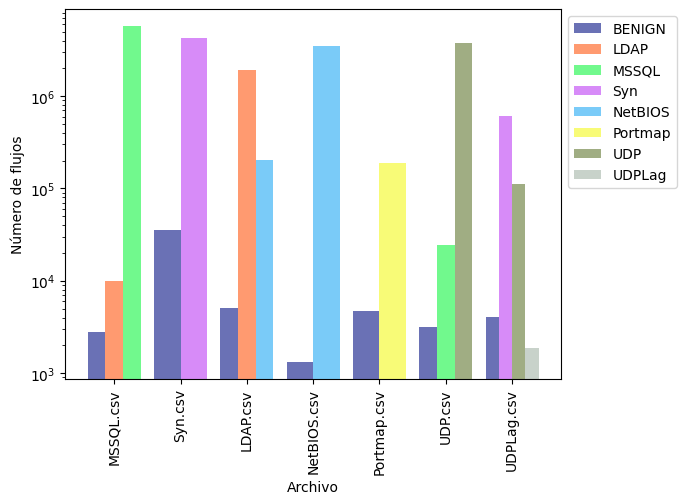
\includegraphics[width=\linewidth]{media/cicddos_2019_csv_03-11_file_results.png}
      \captionsetup{justification=centering}
      \caption{Número de flujos por archivo de las trazas de noviembre 3}\label{fig:cicddos_2019_csv_03-11_file_results}
    \endminipage\hfill
    \minipage{0.49\textwidth}
      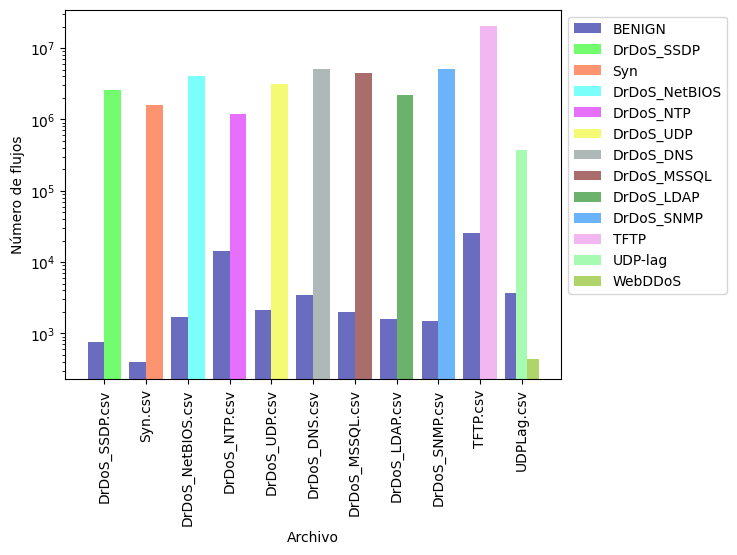
\includegraphics[width=\linewidth]{media/cicddos_2019_csv_01-12_file_results.png}
      \captionsetup{justification=centering}
      \caption{Número de flujos por archivo de las trazas de diciembre 1}\label{fig:cicddos_2019_csv_01-12_file_results}
    \endminipage\hfill
\end{figure}

\begin{figure}[!htb]
    \begin{center}
        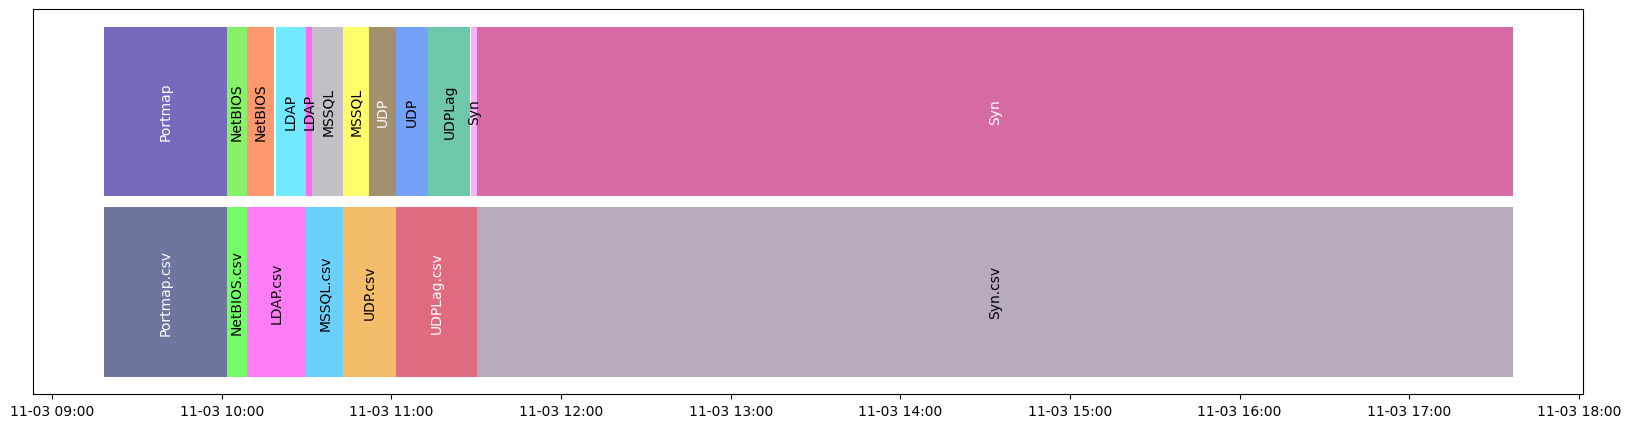
\includegraphics[width=1\linewidth]{media/cicddos_2019_csv_03-11_timeline.png}
    \end{center}
    \captionsetup{justification=centering}
    \caption{Línea temporal de las trazas de noviembre 3 con los archivos (debajo) y los rangos de ataques en estos (arriba)}\label{fig:cicddos_2019_csv_03-11_timeline}
\end{figure}
\begin{figure}[!htb]
    \begin{center}
        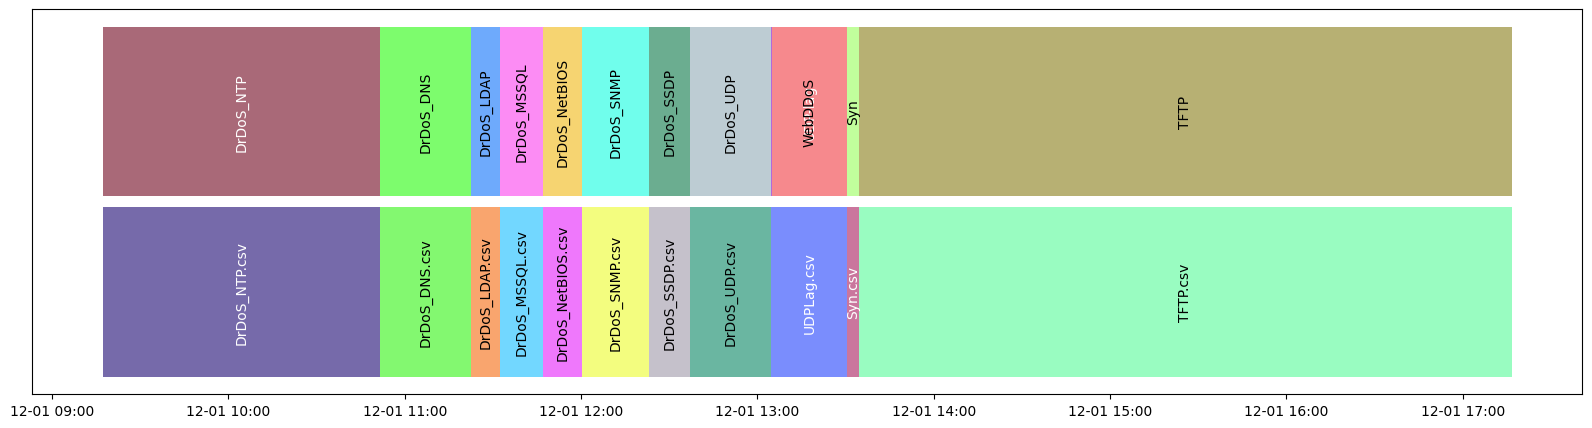
\includegraphics[width=1\linewidth]{media/cicddos_2019_csv_01-12_timeline.png}
    \end{center}
    \captionsetup{justification=centering}
    \caption{Línea temporal de las trazas de diciembre 1 con los archivos (debajo) y los rangos de ataques en estos (arriba)}\label{fig:cicddos_2019_csv_01-12_timeline}
\end{figure}

%\begin{figure}[!htb]
%    \minipage{1\textwidth}
%      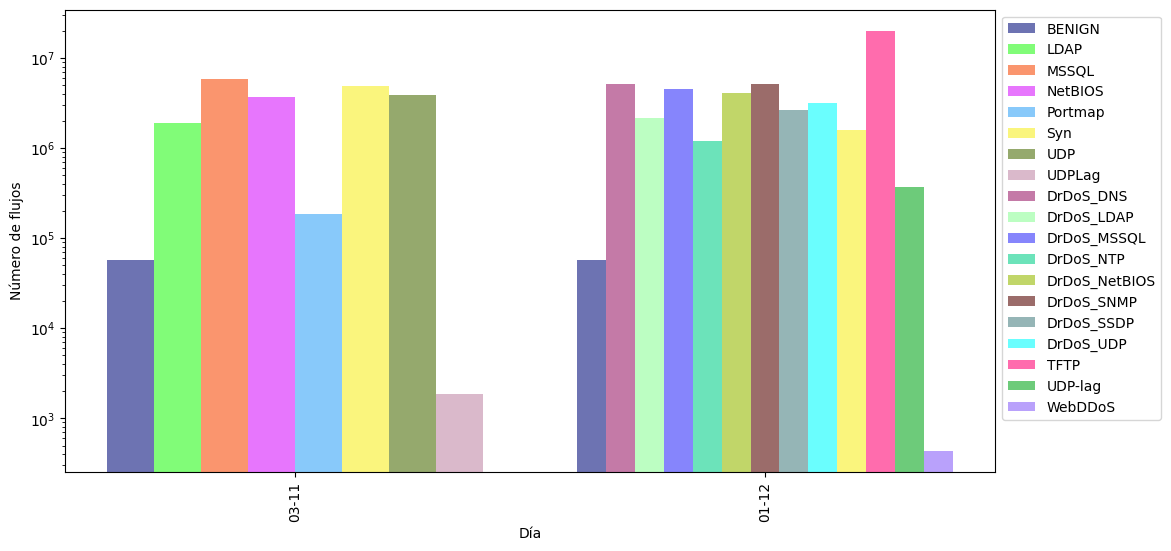
\includegraphics[width=\linewidth]{media/cicddos_2019_csv_day_results.png}
%      \captionsetup{justification=centering}
%      \caption{Número de flujos por archivo de las trazas de noviembre 3}\label{fig:cicddos_2019_csv_day_results}
%    \endminipage
%\end{figure}

\subsubsection{Contenidos pcaps}

El dataset CICDDos2019 ofrece un conjunto de trazas de red de los dos días en los que se generaron datos. Para el primer día (3 de noviembre), hay 145 archivos de unos 190.7 MiB cada uno y un último de 66.5 MiB. Para el segundo día (1 de diciembre), se ofrecen 818 archivos de 190.7 MiB cada uno y uno adicional de 3.7 MiB. En ambos casos, si intentamos abrir el último paquete con Wireshark o generamos cualquier análisis a través de tshark, se nos notifica que el paquete se encuentra 'cortado'. Esto es quizá causado porque, en el momento de generar las trazas, se cortó el proceso de captura precipitadamente. Los scripts utilizados para la extracción de datos es \texttt{extract\_info\_cicddos\_2019\_pcaps\_tshark.sh} y el utilizado para la representacion de estos es \texttt{evaluate\_info\_cicddos\_2019\_pcaps\_tshark.py} disponibles en TODO DEFINIR.

En los pcap, aparecen más direcciones IP en la red del testbed (192.\-168.\-50.\-0/24) de las mencionadas en la información ofrecida en la web del dataset. Concretamente, tenemos que en el primer día aparecen adicionalmente 192.\-168.\-50.\-4, 192.\-168.\-50.\-9 192.\-168.\-50.\-253 y 192.\-168.\-50.\-254. En el segundo día, tenemos que aparecen 192.\-168.\-50.\-253 y 192.\-168.\-50.\-254 además del posible router con IP 192.\-168.\-50.\-1. Adicionalmente, en ambos casos aparece la IP de broadcast (192.\-168.\-50.\-255). Respecto al número de direcciones IP únicas, podemos ver que en el primer día aparecen 1321 y en el segundo 640, teniendo en total 1723 únicas en el transcurso de los dos días. 

Se han generado histogramas con la distribución de la duración de los flujos, número de tramas y número de bytes para poder compararlos con los futuros resultados de la herramienta y comprobar que son consistentes. Como podemos ver en la Figura \ref{fig:cicddos_2019_pcap_duration_distribution}, hay muchos flujos los cuales su duración es relativamente corta y luego hay cierta variedad de flujos de mayor duración. Para el caso de las tramas, podemos observar en la Figura \ref{fig:cicddos_2019_pcap_frames_distribution} que en su mayoría se concentran entre 1 y 1000 tramas y a continuación se reduce drásticamente la cantidad, aunque hay un grupo de flujos los cuales se comprenden entre 10 000 y 100 000. En la Figura \ref{fig:cicddos_2019_pcap_bytes_distribution}, podemos ver que tenemos un caso similar, la mayoría se concentra en las partes bajas, después decrece y hay un grupo numeroso separado el cual realiza una gran transferencia de datos.

\begin{figure}[H]
    \begin{center}
        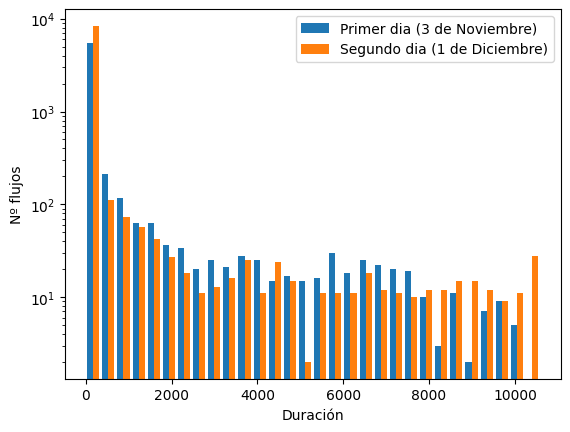
\includegraphics[width=0.49\linewidth]{media/cicddos_2019_pcap_duration_distribution.png}
    \end{center}
    \captionsetup{justification=centering}
    \caption{Distribución duraciones de flujos en CICDDos2019}\label{fig:cicddos_2019_pcap_duration_distribution}
\end{figure}

\begin{figure}[H]
    \minipage{0.49\textwidth}
      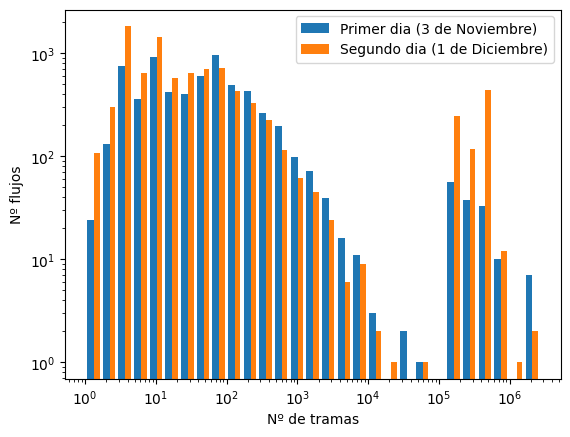
\includegraphics[width=\linewidth]{media/cicddos_2019_pcap_frames_distribution.png}
      \captionsetup{justification=centering}
      \caption{Distribución número de tramas en flujos en CICDDos2019}\label{fig:cicddos_2019_pcap_frames_distribution}
    \endminipage\hfill
    \minipage{0.49\textwidth}
      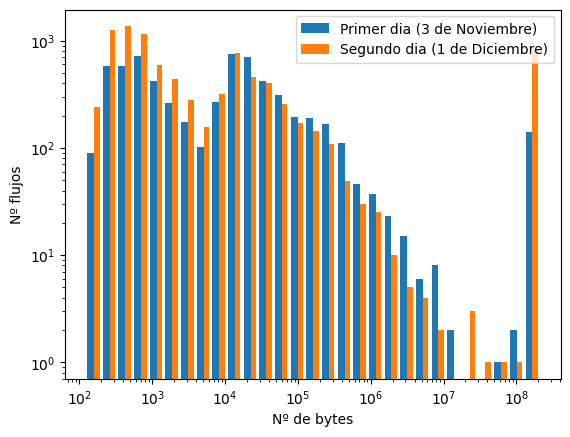
\includegraphics[width=\linewidth]{media/cicddos_2019_pcap_bytes_distribution.png}
      \captionsetup{justification=centering}
      \caption{Distribución número de bytes en flujos en CICDDos2019}\label{fig:cicddos_2019_pcap_bytes_distribution}
    \endminipage\hfill
\end{figure}

Si miramos la cantidad de información transmitida por las diferentes capas de red y de transporte en la tabla \ref{table:cicddos2019protocols}, podemos ver cómo la mayor parte del tráfico consiste en UDP, TCP y otro que tshark no ha podido identificar (data). De los 174.8 GiB transmitidos en total, menos de 10 MiB consisten en tráfico no IPv4. Adicionalmente, un 66.01\% de este tráfico es específicamente UDP, haciendo uso de posibles diversos protocolos en la siguiente capa. Es posible que la cantidad de protocolos sea engañosa, ya que es posible que este número haya sido exagerado a causa de ataques de escaneo en el dataset. Los otros dos puestos sobre la capa de red, consisten en 57.1 GiB (32.66\%) que tshark no pudo identificar y 2.2GiB (1.25\%) de tráfico TCP. 

%Generated with /workspaces/tfg/scripts/evaluate_info_cicddos_2019_pcaps_tshark.py
\begin{table}[H]
    \begin{center}
        \begin{tabular}{|c c c | c c c|} 
            \hline
            \textbf{L0} & \textbf{L1} & \textbf{L2} & \textbf{Tramas} & \textbf{Bytes} & \textbf{Nº subprotocolos}\\
            \hline\hline
eth &- &- & 3.12e+08 & 174.8GiB & 5 \\
eth &ip &- & 3.12e+08 & 174.8GiB & 7 \\
eth &ip &data & 4.44e+07 & 57.1GiB & 0 \\
eth &ip &udp & 2.42e+08 & 115.4GiB & 187 \\
eth &ip &icmp & 2.01e+05 & 29.9MiB & 64 \\
eth &ip &tcp & 2.56e+07 & 2.2GiB & 7 \\
eth &ip &ospf & 4.42e+04 & 4.0MiB & 0 \\
eth &ip &igmp & 1.00e+02 & 5.9KiB & 0 \\
eth &ip &rsvp & 2.00e+00 & 260.0B & 0 \\
eth &llc &- & 3.54e+04 & 3.0MiB & 3 \\
eth &llc &stp & 2.93e+04 & 1.8MiB & 0 \\
eth &llc &dtp & 3.90e+03 & 228.8KiB & 0 \\
eth &llc &cdp & 2.17e+03 & 977.2KiB & 0 \\
eth &ipv6 &- & 2.00e+04 & 2.9MiB & 2 \\
eth &ipv6 &udp & 1.54e+04 & 2.5MiB & 5 \\
eth &ipv6 &icmpv6 & 4.59e+03 & 418.5KiB & 0 \\
eth &arp &- & 9.14e+03 & 535.6KiB & 0 \\
eth &lldp &- & 1.22e+02 & 7.1KiB & 0 \\
            \hline
        \end{tabular}
    \end{center}
    \caption{Primeras tres capas de protocolos identificados en CICDDos2019}
    \label{table:cicddos2019protocols}
\end{table}


\subsection{BoT-IoT}

(por hacer)

\subsection{TON-IoT}

(por hacer)

\subsection{UNSW-NB15}

(por hacer)


\section{Formatos y protocolos de red}

En esta sección definiremos los diferentes protocolos y formatos de red que serán tenidos en cuenta. Concretamente, veremos el formato 'libpcap' en el que las trazas de red son guardadas, las capas de enlace de Ethernet y Linux Cooked Capture v1 (SLL), las capas de red IPv4 e IPv6 y las capas de transporte UDP y TCP.

\subsection{libpcap}

\subsubsection{Descripción}

El formato libpcap es un formato de captura de trazas de red utilizado en TcpDump, WinDump, Wireshark, entre otros \cite{pcapfileformatwireshark} \cite{pcapfileformatrfc}. La estructura general consiste en una cabecera de fichero y a continuación uno cero o más 'Packet Records' o registros de paquetes. Cada uno de estos contiene una cabecera con información de la captura y bytes provenientes del paquete capturado. Adicionalmente, el orden de los campos de los bits dentro de las cabeceras depende del formato nativo de la máquina donde se capturaron los paquetes. 

\subsubsection{Cabecera de fichero}

\begin{figure}[H]
    \begin{center}
        \begin{bytefield}{32}
            \bitheader{0-31} \\
            \bitbox{32}{Número mágico} \\
            \bitbox{16}{Versión mayor} 
            \bitbox{16}{Versión menor} \\
            \bitbox{32}{Reservado 1} \\
            \bitbox{32}{Reservado 2} \\
            \bitbox{32}{Longitud máxima capturada} \\
            \bitbox{3}{FCS} & \bitbox{1}{f}
            \bitbox{28}{Tipo capa de enlace} \\
            \bitheader{0-31} \\
        \end{bytefield}
    \end{center}
    \caption{Formato cabecera archivo libpcap}
    \label{fig:libpcap_file_header}
\end{figure}

El orden de los campos en la cabecera del fichero es como podemos ver en la Figura \ref{fig:libpcap_file_header}. El significado de los campos es el siguiente:

\begin{enumerate}
    \item \textbf{Número mágico}: Permite identificar el archivo como pcap, conocer la precisión de los campos de tiempo y saber el orden de bits de las cabeceras. El valor del campo en hexadecimal es \texttt{0xA1B2C3D4} si tenemos segundos y microsegundos. En caso de que sea \texttt{0xA1B23C4D}, tenemos precisión de nanosegundos en vez de microsegundos. Finalmente, si el primer byte del fichero tiene el valor \texttt{0xA1}, los campos tienen el orden 'big endian' (los bytes más significativos aparecen primero). En el caso opuesto, tienen el orden 'little endian' (los bytes menos significativos aparecen primero).
    \item \textbf{Versión mayor}: Valor no entero representando la versión semántica mayor \cite{preston2013semantic}. La última versión hasta la fecha es 2.
    \item \textbf{Versión menor}: Valor no entero, representando la versión semántica menor \cite{preston2013semantic}. La última versión hasta la fecha es la 4.
    \item \textbf{Reservado 1}: Valor no utilizado en la actualidad. En versiones antiguas se utilizaba para marcar la diferencia de huso horario.
    \item \textbf{Reservado 2}: Valor no utilizado en la actualidad. En versiones antiguas se utilizaba para indicar la precisión de las marcas de tiempo.
    \item \textbf{Longitud máxima capturada}: Número máximo de bytes de los paquetes originales que pueden ser incluidos en la traza de red. Si hay algún paquete que originalmente es más grande que este tamaño, se trunca a la longitud indicada.
    \item \textbf{FCS/f}: si el bit "f" está a 1, los siguientes 3 bits indican el número de bytes de detección de errores añadidos a continuación. 
    \item \textbf{Tipo capa de enlace}: Número identificando el tipo de la capa de enlace utilizado. Algunos ejemplos son 1 para IEEE 802.3 (Ethernet) o 113 para 'Linux Cooked Capture v1' \cite{linktypetcpdump}
\end{enumerate}

\subsubsection{Registro de paquete}

El orden de los campos en la cabecera del fichero es como podemos ver en la Figura \ref{fig:libpcap_file_packet_record}. La marca se encuentra representada como el número de segundos y micro/nanosegundos (dependiendo de la cabecera del fichero) transcurridos desde el 1 de enero de 1970 a las 00:00 UTC. Se incluye el tamaño del paquete original y el capturado, ya que no todos los paquetes de la captura tienen necesariamente el mismo tamaño que el original ni entre ellos.

\begin{figure}[h]
    \begin{center}
        \begin{bytefield}{32}
            \bitheader{0-31} \\
            \bitbox{32}{Marca de tiempo (parte de segundos)} \\
            \bitbox{32}{Marca de tiempo (parte de micro/nanosegundos)} \\ 
            \bitbox{32}{Tamaño del paquete capturado} \\
            \bitbox{32}{Tamaño del paquete original} \\
            \wordbox{3}{Datos del paquete} \\
        \end{bytefield}
    \end{center}
    \caption{Formato registro de paquete archivo libpcap}
    \label{fig:libpcap_file_packet_record}
\end{figure}

\subsection{Ethernet}

por hacer

\subsection{Linux Cooked Capture v1 (SLL)}

por hacer

\subsection{IP versión 4}

por hacer

\subsection{IP versión 6}

por hacer

\subsection{UDP}

por hacer

\subsection{TCP}

por hacer

\section{Software para el desarrollo}

En esta sección resumiremos los diferentes elementos software que serán utilizados para el desarrollo del trabajo. Concretamente, se indicarán los lenguajes de programación utilizados y los programas, además de la razón de su uso.

\subsection{Lenguajes de programación}

\subsubsection{Rust}

Rust es un lenguaje de programación compilado de propósito general y multiparadigma \cite{blandy2017programming} \cite{klabnik2018rust}. Este trata de garantizar que todas las referencias a memoria sean válidas e impedir condiciones de carrera sin tener necesidad de un 'recolector de basura' como Java o Python. Esto lo hace a través de, en el momento de compilación, comprobar que los usos de memoria sean correctos. 

Debido a que garantizar con exactitud si un programa hace uso de la memoria de forma correcta es un reto, el compilador toma una posición más conservadora. En caso de que el programador tenga más información y sepa que un uso de memoria que el compilador rechaza es correcto, existen métodos para hacer que el compilador lo acepte. Ejemplos son el uso de \texttt{unwrap()} para acceder a valores opcionales, el cual, si no contiene el valor esperado, interrumpe el programa en vez de corromper la memoria, o bloques \texttt{unsafe}, donde el programador ha de manualmente comprobar que no se está accediendo a memoria inválida.

Se ha escogido este lenguaje para el desarrollo de la herramienta debido a la capacidad de escribir código de bajo nivel, su alto rendimiento, su énfasis en el código correcto, la calidad de las herramientas asociadas y el gran número de librerías disponibles. 

\subsubsection{Bash}

\color{blue} %TODO remove this when revised

Bash, también conocido como GNU Bash, es un programa Shell y un lenguaje de comandos asociado que formaba originalmente parte del sistema operativo GNU \cite{gnubashweb} \cite{gnubashmanual}. Se puede ejecutar de forma interactiva, donde escribimos los comandos directamente en el terminal, o de manera no interactiva, donde le pasamos un archivo con la lista de comandos a ejecutar. Los comandos pueden ser palabras intrínsecas del lenguaje (\texttt{if}, \texttt{do}, entre otros) o programas para ser ejecutado. Adicionalmente, tiene soporte para bucles, guardar y expandir variables, funciones, listas, ente otros.

Se ha escogido Bash porque es la Shell utilizada por defecto en muchas distribuciones Linux. Con esta, automatizaremos tareas que requieran tratar archivos con herramientas existentes, como por ejemplo \texttt{tshark}.

\subsubsection{Python}

Python es un lenguaje de programación interpretado de propósito general y multiparadigma \cite{aboutpython} \cite{davepython}. Trata de focalizarse en la legibilidad del código y su facilidad de uso en la medida de lo posible. Esto lo hace a través de una librería estándar extensa, una gran cantidad de librerías creadas por la comunidad, tipos dinámicos y un 'recolector de basura' que permite a los desarrolladores no tener que gestionar memoria de forma manual.

Se ha escogido este lenguaje para las tareas que consistan en visualizar y tratar datos, además de las tareas de \gls{ml}, ya que es uno de los lenguajes frecuentemente utilizados para esto. Adicionalmente, las librerías disponibles y la documentación asociada facilitarán su uso.

\subsection{Programas}

\subsubsection{Git}

por hacer

\subsubsection{Docker}

por hacer

\subsubsection{Visual Studio Code}

por hacer


\newpage
\pagestyle{plain}

\chapter{CHAPTER TEST}

TODO
\section{SECTION TEST}

TODO

\subsection{SUBSECTION TEST}

TODO

\newpage
\pagestyle{plain}

\chapter{CONCLUSIONES}

Como recapitulación del trabajo, primero haremos un recuento aproximado de los posibles costes que se hubiesen incurrido en caso de haber sido un proyecto empresarial. Después de esto, se hará un análisis de los resultados generales obtenidos y continuaremos con indicaciones sobre posible trabajo futuro. Finalmente, concluiremos con los agradecimientos.

\section{Costes}

\begin{table}[H]
  \centering
  \begin{tabular}{|l | r |}
      \hline
      \rowcolor{lightgray} \textbf{Tarea}                & \textbf{Horas}       \\  
      \hline
      \rowcolor{lightgray} Gestión del proyecto     &  45                  \\
      Reuniones de seguimiento                      &  35                  \\
      Gestión de las tareas                         &   5                  \\
      Planificación temporal                        &   5                  \\  
      \hline
      \rowcolor{lightgray} Investigación            & 125                  \\
      Herramientas de extracción de características  &  75                  \\
      Conjuntos de datos                            &  30                  \\
      Formatos y protocolos de red                  &  10                  \\
      Otro software utilizado                       &  10                  \\
      \hline
      \rowcolor{lightgray} Desarrollo                & 220                  \\
      Programación de la herramienta                & 110                  \\
      Extensión de la librería de código abierto    &  30                  \\
      Modelos de ML                                 &  80                  \\
      \hline
      \rowcolor{lightgray} Documentación            & 145                  \\
      Redacción de la memoria                       & 110                  \\
      Artículo                                      &  20                  \\
      Presentación                                  &  15                  \\
      \hline
      \rowcolor{lightgray} Total                    & 535                  \\
      \hline
  \end{tabular}
  \caption{Horas aproximadas dedicadas a diferentes partes del proyecto}
  \label{table:horasdedicadas}
\end{table}

En la Tabla \ref{table:horasdedicadas} se puede observar un desglose aproximado de las horas utilizadas para el desarrollo del proyecto. Debido a que se estaban cursando asignaturas y colaborando con el grupo de Investigación CRAAX al mismo tiempo, es posible que haya habido interferencias y el número real sea inferior o superior. 

Respecto al coste por horas, podemos ver en la Tabla \ref{table:salarios} un posible coste de la realización del trabajo, tomando como referencia diferentes salarios medios según la tarea realizada. El total asciende a 13 447.47, aunque los tiempos requeridos y los salarios podrían haber sido distintos en un entrono empresarial.

\begin{table}[H]
  \centering
  \begin{tabular}{|l | c c c |}
      \hline
      \rowcolor{lightgray} \textbf{Rol} & \textbf{Salario medio por hora}            & \textbf{Horas totales} & \textbf{Coste total} \\ \hline
      Ingeniero de proyectos            & 14.10 € \cite{salarioingenierodeproyectos} &  45                    &    634.5  €          \\
      Programador                       & 14.36 € \cite{salarioprogramador}          & 235                    &  9 111.42 €          \\
      Científico de datos               & 20.64 € \cite{salariodatasci}              & 110                    &  2 270.4  €          \\
      Redactor técnico                  &  9.87 € \cite{salarioredactor}             & 145                    &  1 431.15 €          \\ \hline
      \rowcolor{lightgray}              &                                           &                        & \textbf{13 447.47 €}  \\
      \hline
  \end{tabular}
  \caption{Cálculo coste horas por tarea realizada}
  \label{table:salarios}
\end{table}

No se han incurrido en costes de licencias, ya que todo el software utilizado ha sido gratuito o de código libre. Para el caso del ordenador de sobremesa, donde se han ejecutado los algoritmos y se ha hecho la mayor parte del desarrollo, está valorado en unos 2 500 €.

Si hacemos la suma total, el coste total sería de unos 16 000 €. Cabe notar que esta suma se ha realizado sin tener en cuenta costes indirectos como la factura eléctrica.

\section{Análisis resultados}

por hacer

\section{Trabajo futuro}

por hacer

\section{Agradecimientos}

por hacer

\newpage
\pagestyle{plain}

\phantomsection\addcontentsline{toc}{chapter}{AGRADECIMIENTOS}
\chapter*{AGRADECIMIENTOS}

TODO


% Bibliography
\newpage
\pagestyle{plain}

\phantomsection\addcontentsline{toc}{chapter}{BIBLIOGRAFÍA}
\chapter*{BIBLIOGRAFÍA}

TODO

\newpage
\pagestyle{plain}

\pdfbookmark[-1]{ANEXOS}{ANEXOS}

\cftaddtitleline{toc}{chapter}{ANEXO 1}{}
\pdfbookmark[0]{ANEXO 1}{ANEXO 1}
\chapter*{ANEXO 1}
\setcounter{page}{0}

TODO

\cftaddtitleline{toc}{chapter}{ANEXO 2}{}
\pdfbookmark[0]{ANEXO 2}{ANEXO 2}
\chapter*{ANEXO 2}
\setcounter{page}{0}

TODO


\end{document}
